\section{Methods}

\subsection{Model processes}

Figure \ref{fig:process} describes the processes modeled. \textit{Usual care} may be provided by first admission either at a \textit{primary stroke centre} providing IVT only (with onward transfer to comprehensive stroke centre for MT), or a \textit{comprehensive stroke centre} providing both IVT and MT. The alternative pathway of a \textit{mobile stroke unit} involved the mobile stroke unit providing on-scene IVT, followed by transfer to the closest comprehensive stroke centre for MT.

Unless specified otherwise, it is assumed that mobile stroke units are located at comprehensive stroke centres.

Geographic analysis was undertaken at Lower Super Output Area (LSO) level. Travel times from each LSOS to all hospitals and travel times between hospitals have been estimated using Open Street Map data, with results calibrated against Google Maps. Travel times have been made available (\url{https://gitlab.com/michaelallen1966/1811_lsoa_to_acute_hospital_travel}).

\begin{figure}
    \centering
    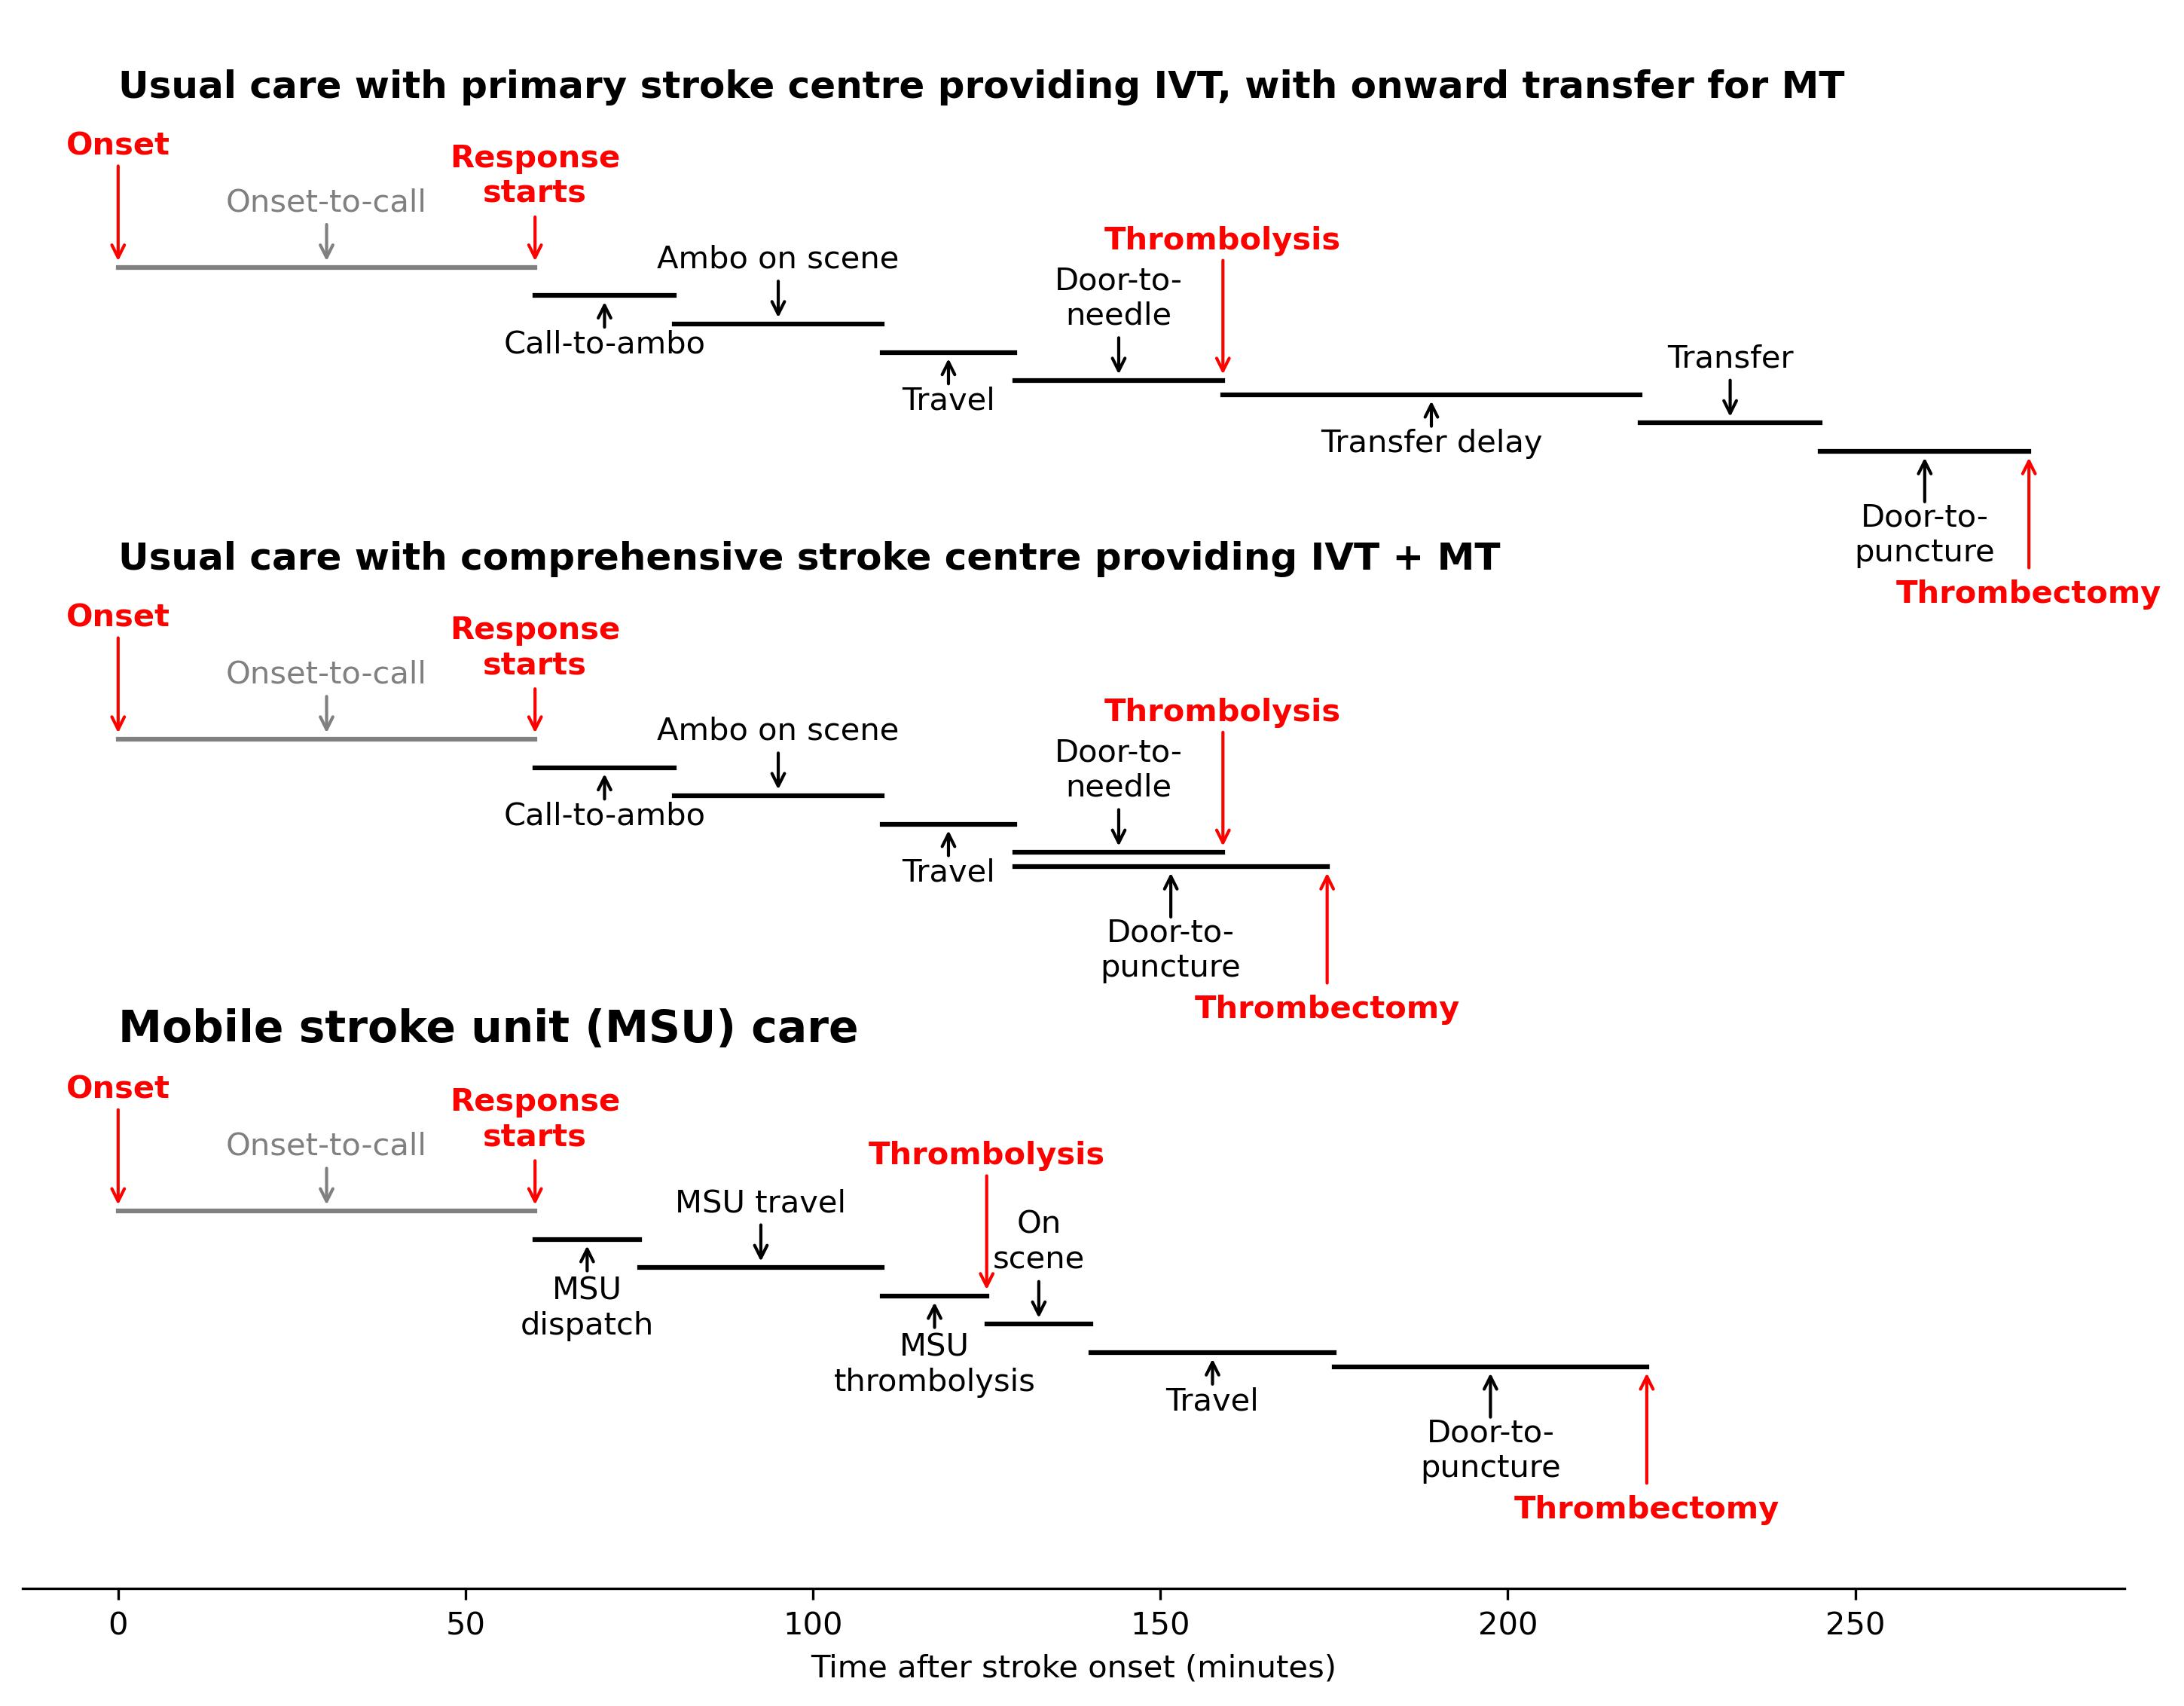
\includegraphics[width=0.85\linewidth]{images/stroke_treatment.jpg}
    \caption{Processes modeled for provision of IVT and MT. Top: First admission to a primary stroke centre providing IVT, followed by transfer to a comprehensive stroke centre for MT. Middle first admission to a comprehensive stroke centre providing both IVT and MT. }
    \label{fig:process}
\end{figure}

\subsection{Outcome modeling}

\subsection{Scenario analysis}

Scenario analysis was undertaken to investigate how model parameters

\subsection{Geographic analysis}



